\documentclass[12pt,hyperref={pdfpagelabels=false},notes=show,aspectratio=169]{beamer}

\usetheme[]{FFF}

% Bugfix for pdfpagelables=false
\providecommand\thispdfpagelabel[1]{}

% Standard packages

\usepackage[english,ngerman]{babel}
\usepackage[utf8]{inputenc}
\usepackage{times}

% Setup TikZ

\usepackage{tikz}
\usetikzlibrary{arrows}
\tikzstyle{block}=[draw opacity=0.7,line width=1.4cm]

% Text \us
\usepackage{textcomp}
\usepackage{mathcomp}

% Textpos
\usepackage[absolute,overlay]{textpos}
\setlength{\TPHorizModule}{\paperwidth}
\setlength{\TPVertModule}{\paperheight}

% Blitz-Symbol
\usepackage{stmaryrd}

% Tabellen
\usepackage{multirow}
\usepackage{array}
\usepackage{colortbl}
\definecolor{lightblue}{rgb}{ 0.55, 0.55, 1.00}
\definecolor{lightred}{rgb}{  1.00, 0.35, 0.35}
\definecolor{lightgreen}{rgb}{0.50, 1.00, 0.50}
\newcommand{\ccg}{\cellcolor{lightgreen}}
\newcommand{\ccr}{\cellcolor{lightred}}
\newcommand{\ccb}{\cellcolor{lightblue}}

% Listings
\usepackage{listings}

\setlength{\parindent}{0cm}

% Stroke
\usepackage{ulem}

% vc
\input{vc.tex}

%%%%%%%%%%%%%%%%%%%%%% /LAYOUT %%%%%%%%%%%%%%%%%%%%%%%%%%%%


% Author, Title, etc.

\title{Willkommen zum \#18FFF}

\subtitle{Freifunk Festival 2018}

\author[Tim Niemeyer]{Tim Niemeyer {\tiny \textless{}tim@tn-x.org\textgreater{}}\texorpdfstring{\tiny \\
                        7E7B~3401~42AA~9295~B8F2~~~6C4C~20A9~F38D~2945~ECB5\\\\
                        https://github.com/RedDog99/fff-vortrag.git~~~~\VCRevisionMod}{}}

\date[05.10.2018]{5.10.2018}

\newcommand{\zb}{z.\,B.\@}
\newcommand{\us}{~\textmu{}s}
\newcommand{\uv}{~\textmu{}V}
\newcommand{\ms}{~ms}

\begin{document}

\usebackgroundtemplate{
\includegraphics[height=\paperheight,width=\paperwidth]{slides_background_title}}

\beamertemplatenavigationsymbolsempty
\begin{frame}[plain,squeeze]
	\maketitle
\end{frame}\addtocounter{framenumber}{-1}

\usebackgroundtemplate{
\includegraphics[height=\paperheight,width=\paperwidth]{slides_background}}

\begin{frame}{Willkommen}
    \begin{center}
        Willkommen
    \end{center}
\end{frame}

%%%%%%%%%%%%%%%%%%%%%% CONTENT %%%%%%%%%%%%%%%%%%%%%%%%%%%%

\section{18fff}

\begin{frame}{Freifunk Festival 2018}
    \begin{itemize}
        \item Geboren in Oldenburg im Jahre 2017
        \item Mal nicht in Berlin
        \item Time-division-denzentral: Jedes Jahr wo anders
    \end{itemize}
\end{frame}

\begin{frame}{Der Ablauf}
    \begin{itemize}
        \item Es gibt keinen festen Ablauf
        \item Das Event lebt vom Mitmixen
    \end{itemize}
    \url{https://wiki.freifunk.net/Freifunk\_Festival\_2018/Timetable}
\end{frame}

\begin{frame}{Franziane}
    \begin{itemize}
        \item Franziane ist uns zugelaufen
        \item Freifunk Festival Maskottchen
        \item Immer nett zu Franziane sein
    \end{itemize}
    \begin{textblock*}{0.4\textwidth}(0.6\textwidth,0.05\textheight)
        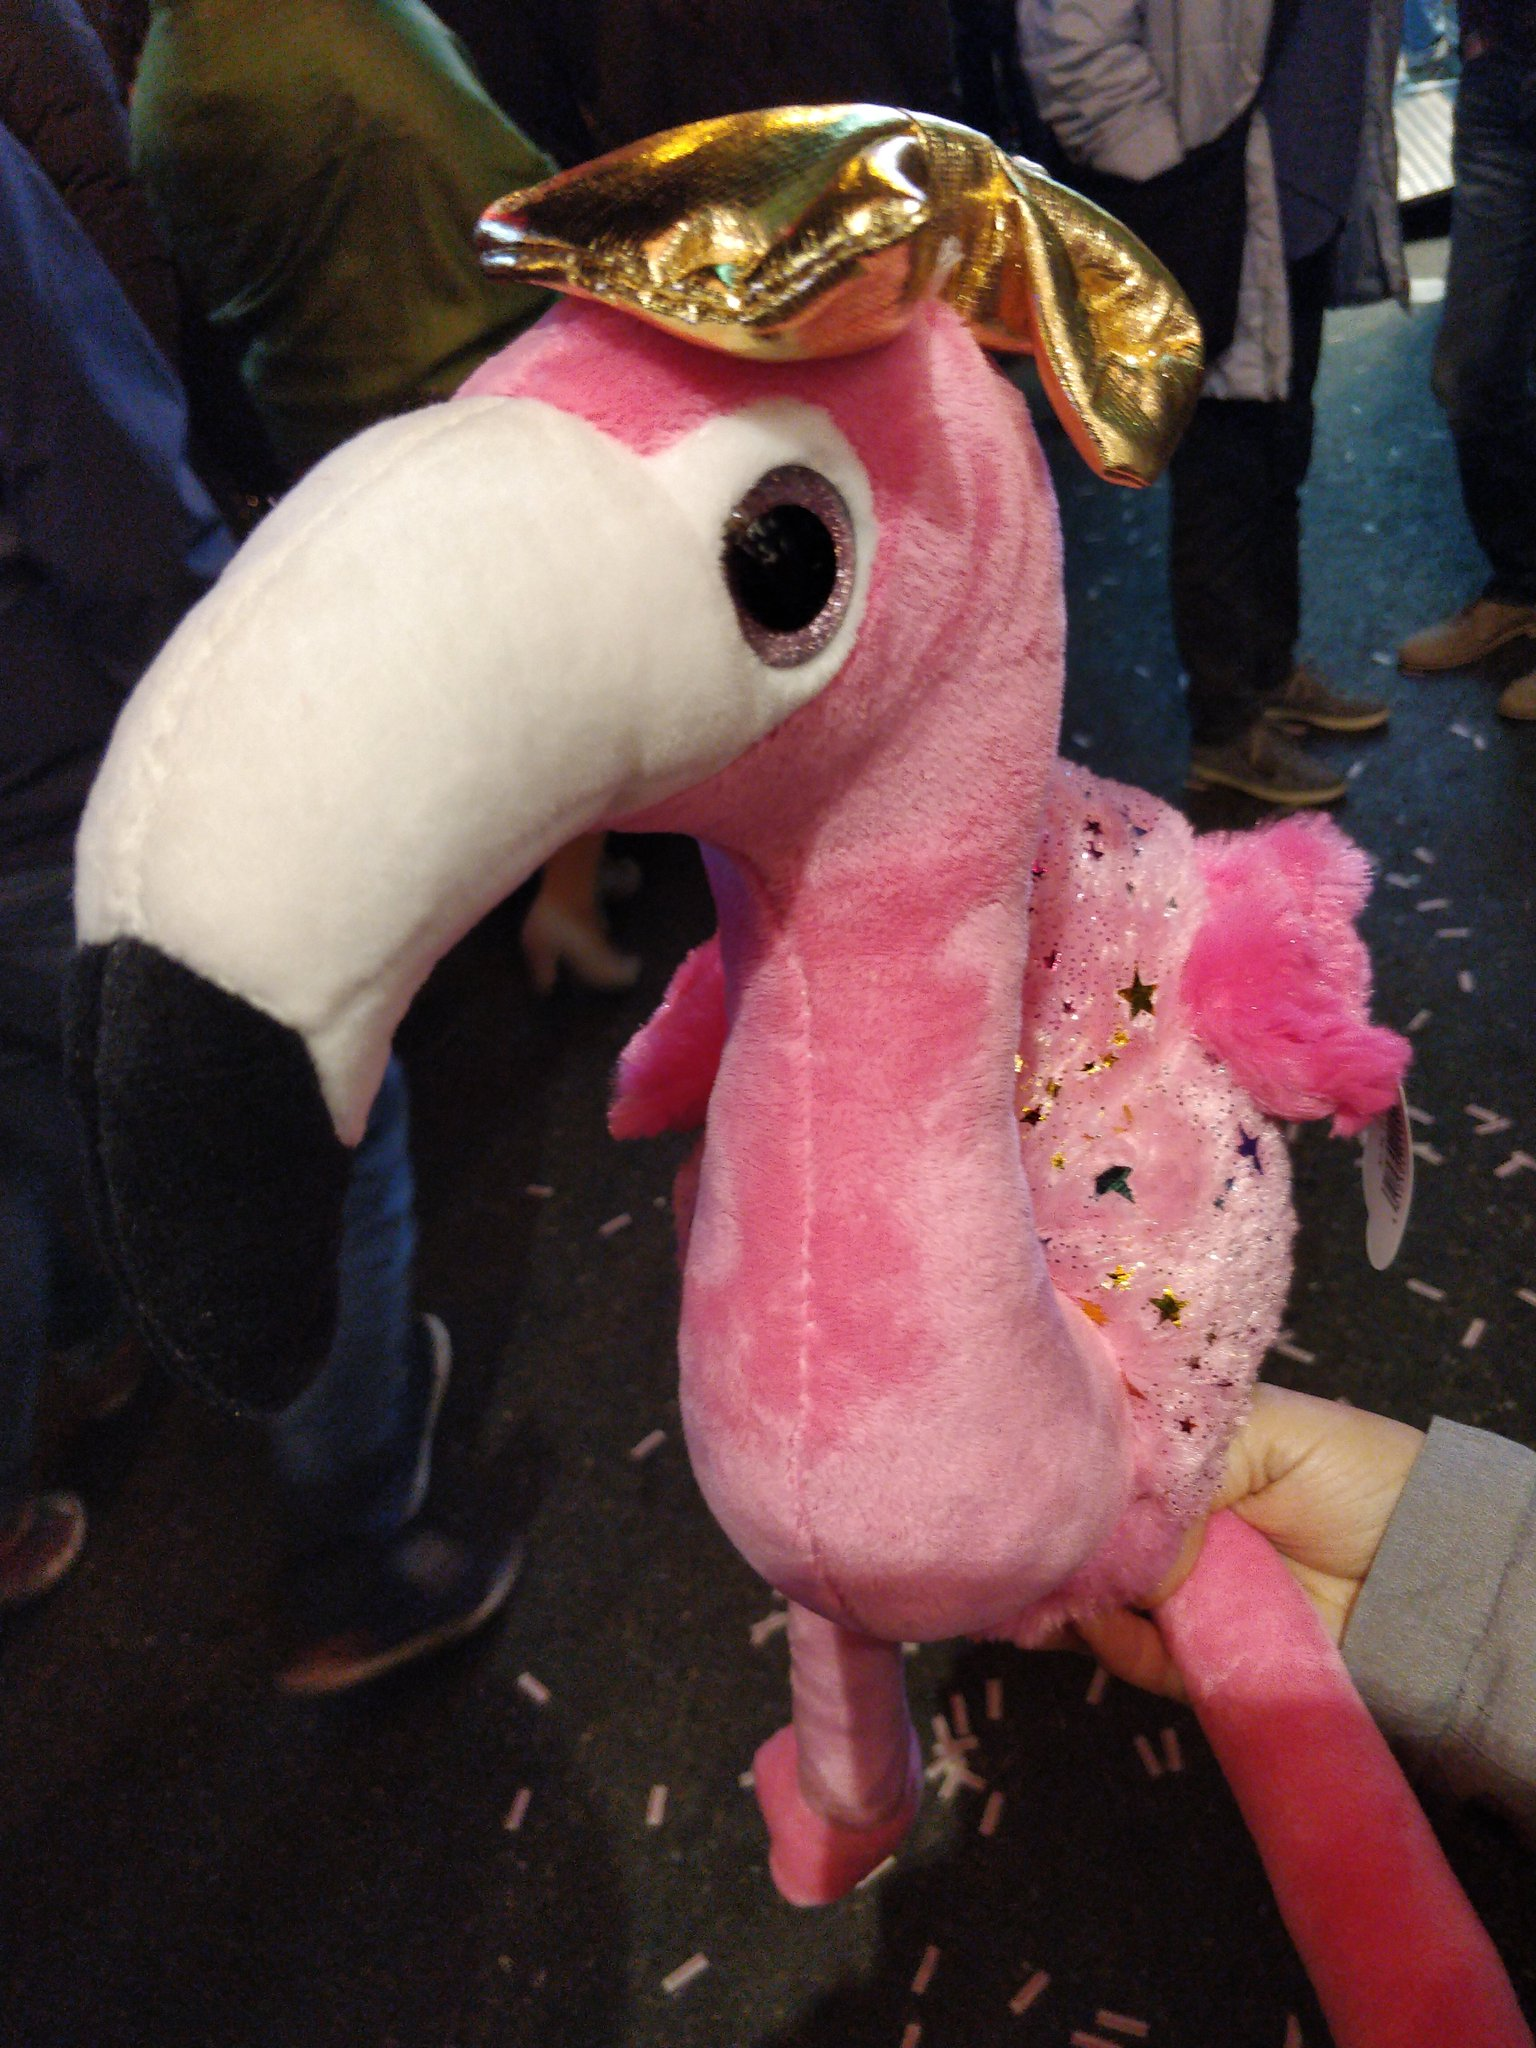
\includegraphics[keepaspectratio,height=0.9\textheight]{img/franziane}
    \end{textblock*}
\end{frame}

\begin{frame}{Wichtige Dates}
    \begin{itemize}
        \item Socialising
        \begin{itemize}
            \item Freitag ab 22 Uhr in der Lounge
            \item Samstag ab 20:30 entweder
            \begin{itemize}
                \item Lounge
                \item Stadtfest
            \end{itemize}
        \end{itemize}
        \item Deadlines
        \begin{itemize}
            \item Anmeldung Samstag-Frühstück: Freitag 22 Uhr
            \item Anmeldung Sonntag-Frühstück: Samstag 16 Uhr
        \end{itemize}
    \end{itemize}
\end{frame}

\section{Meehäusle}

\begin{frame}{Das Meehäusle}
    \begin{itemize}
        \item Vereinsheim von F3 Netze e.V.
    \end{itemize}
\end{frame}

\begin{frame}{Essen / Trinken}
    \begin{itemize}
        \item Meehäusle
        \begin{itemize}
            \item Frühstück-Buffet Samstag 09:00 - 11:30
            \begin{itemize}
                \item 5 € / Anmeldung bis heute 22:00!
            \end{itemize}
            \item Weißwurst-Frühstück Sonntag 10:00 - 10:30
            \begin{itemize}
                \item 5 € / Anmeldung bis heute 16:00!
            \end{itemize}
            \item Warme Küche von 11 - 21 Uhr
            \begin{itemize}
                \item Karte liegt aus
            \end{itemize}
            \item Gemeinsam grillen möglich
        \end{itemize}
        \item Other
        \begin{itemize}
            \item Pizza bestellen (Internet o. an der Theke)
            \item .. eigenes Essen ..
        \end{itemize}
    \end{itemize}
\end{frame}


\section{F3 Netze e.V.}

\begin{frame}{}
    \begin{center}
        F3 Netze e.V.
     \end{center}
\end{frame}

\begin{frame}{Verein ?}
    \begin{columns}[T]
        \begin{column}{0.45\textwidth}
            Was ist F3 Netze e.V.
            \begin{itemize}
                \item Infrastrukturverein
                \item IP-Ressourcen
                \item Provider $\rightarrow$ Traffic ''ausleiten''
                \item Standortüberlassungen
                \item Teilnehmer vom Freifunk Netz
                \item \underline{Keine} Community vertretung
            \end{itemize}
        \end{column}
        \begin{column}{0.45\textwidth}
            Was tut F3 Netze e.V.
            \begin{itemize}
                \item Freifunk Gateways
                \item Richtfunk-Standorte
                \item Tor Exit
                \item BFWA Frequenzen
            \end{itemize}
        \end{column}
    \end{columns}
\end{frame}

\begin{frame}{St. Paul}
    \center
    \only<1>{
        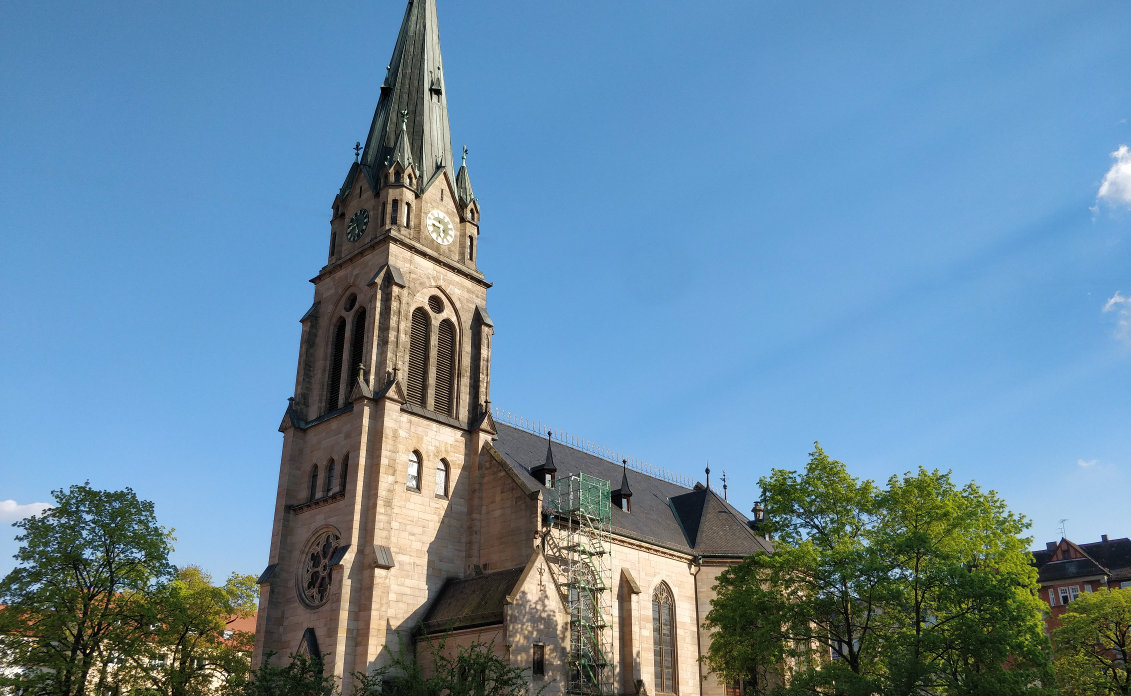
\includegraphics[height=0.86\textheight]{img/stpaul-turm}
    }
    \only<2>{
        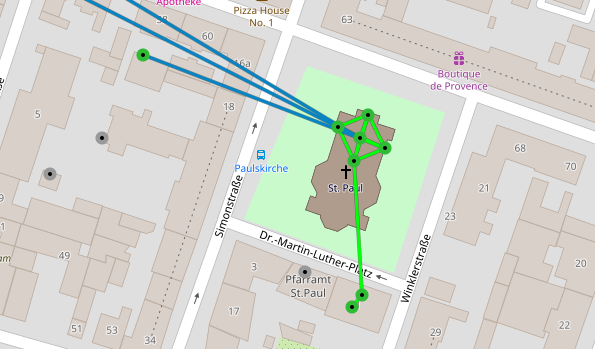
\includegraphics[height=0.86\textheight]{img/stpaul-karte}
    }
    \only<3>{
        \includegraphics[width=0.96\textwidth]{img/dia/stpaul}
    }
    \only<4>{
        ~
        \hfill
        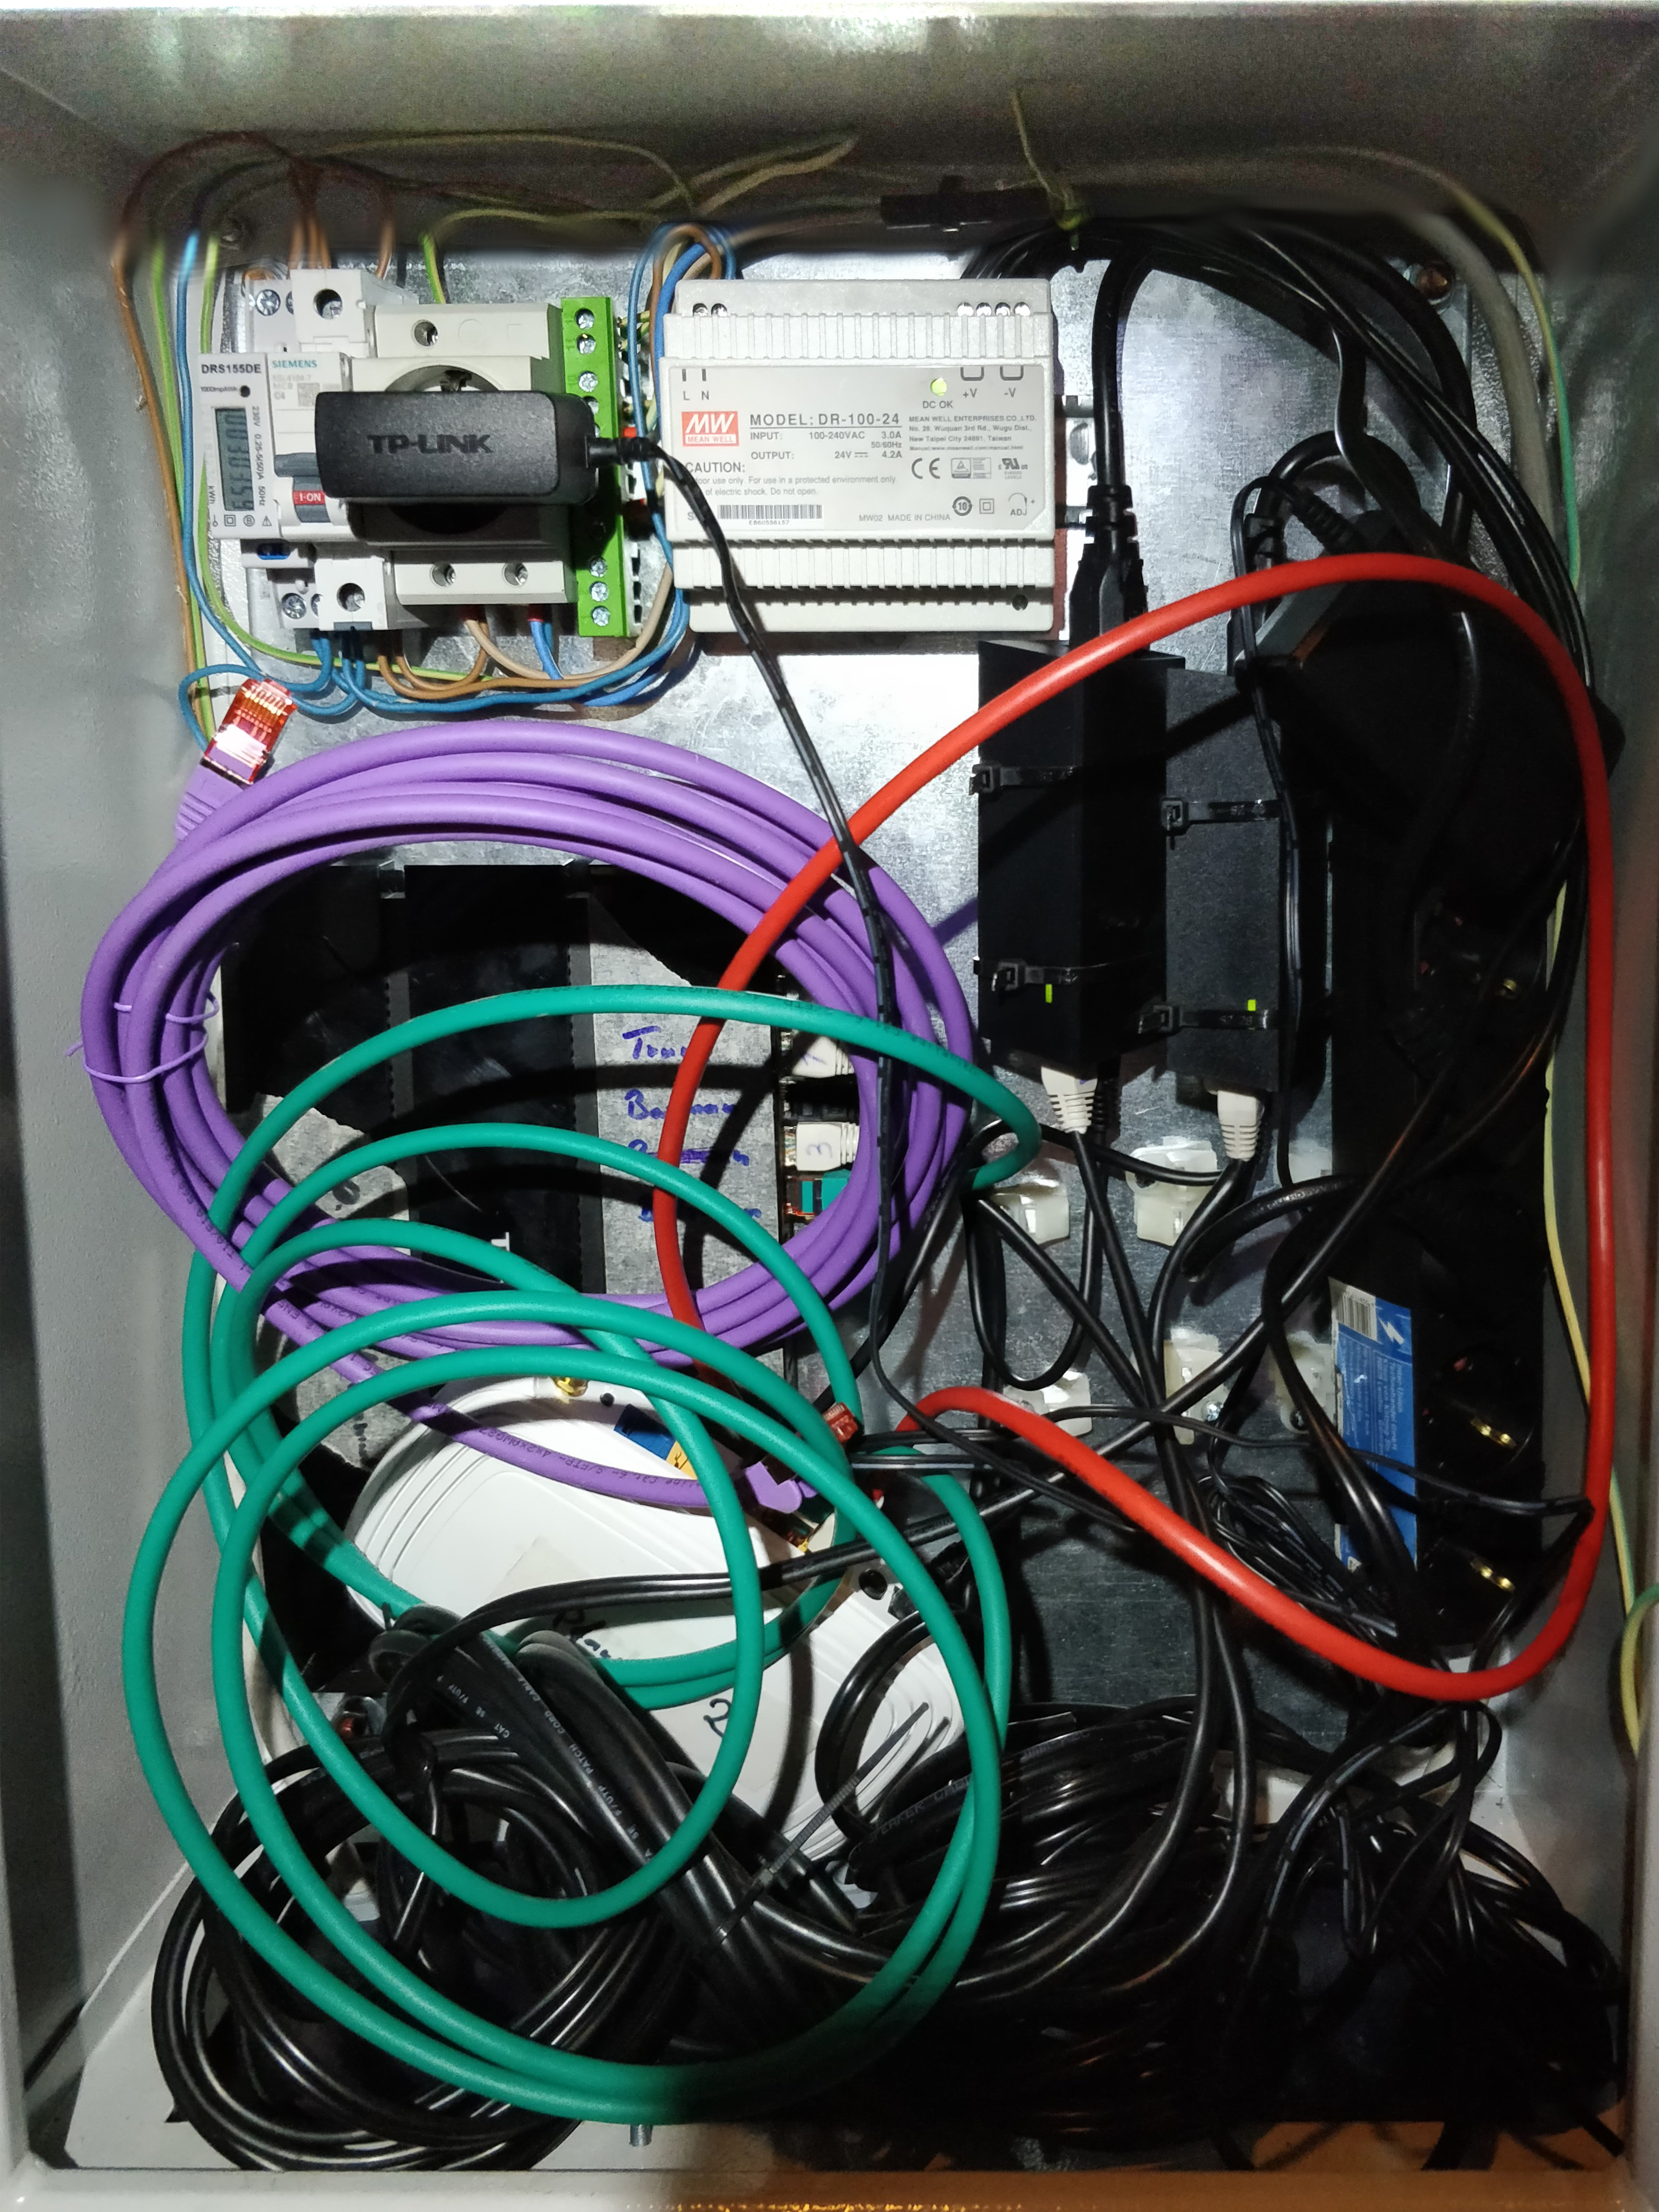
\includegraphics[height=0.86\textheight]{img/stpaul-kasten}
        \hfill
        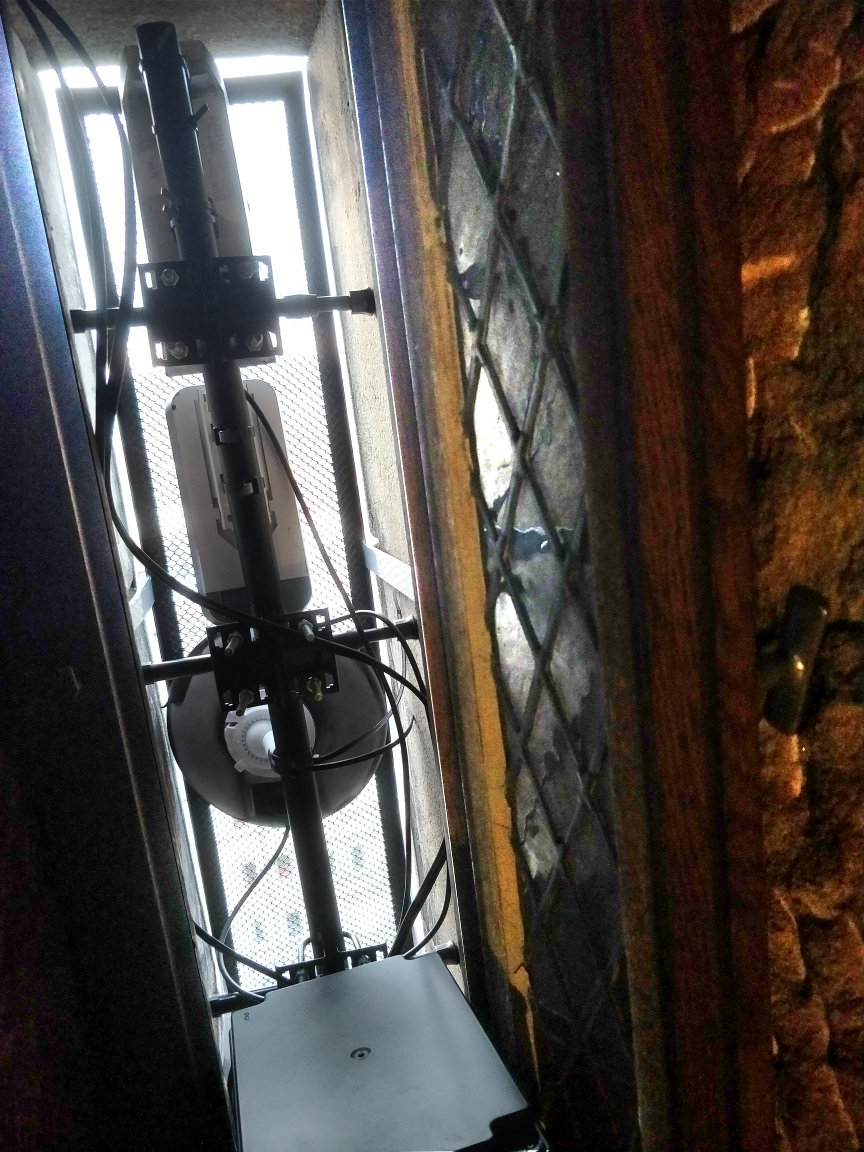
\includegraphics[height=0.86\textheight]{img/stpaul-fenster}
        \hfill
        ~
    }
\end{frame}

\begin{frame}{Z-Bau}
    \only<1>{
        \begin{itemize}
            \item IP-Ressourcen von den Zwiebelfreunde e.V.
            \begin{itemize}
                \item AS205100
                \item 185.220.100.0/24
                \item 2a0b:f4c0::/32
            \end{itemize}
            \item Glasfaser zum Nürnberg Internet Exchange (N-IX)
            \item 10 GBit/s Port von 
\includegraphics[height=1em]{img/proact}
            \item 800 MBit/s Transit
            \item $\sim$38 Peerings
            \item[$\rightarrow$] Aktuell ~400 MBit/s Tor Exit Traffic
        \end{itemize}
    }
    \only<2>{
        \center
        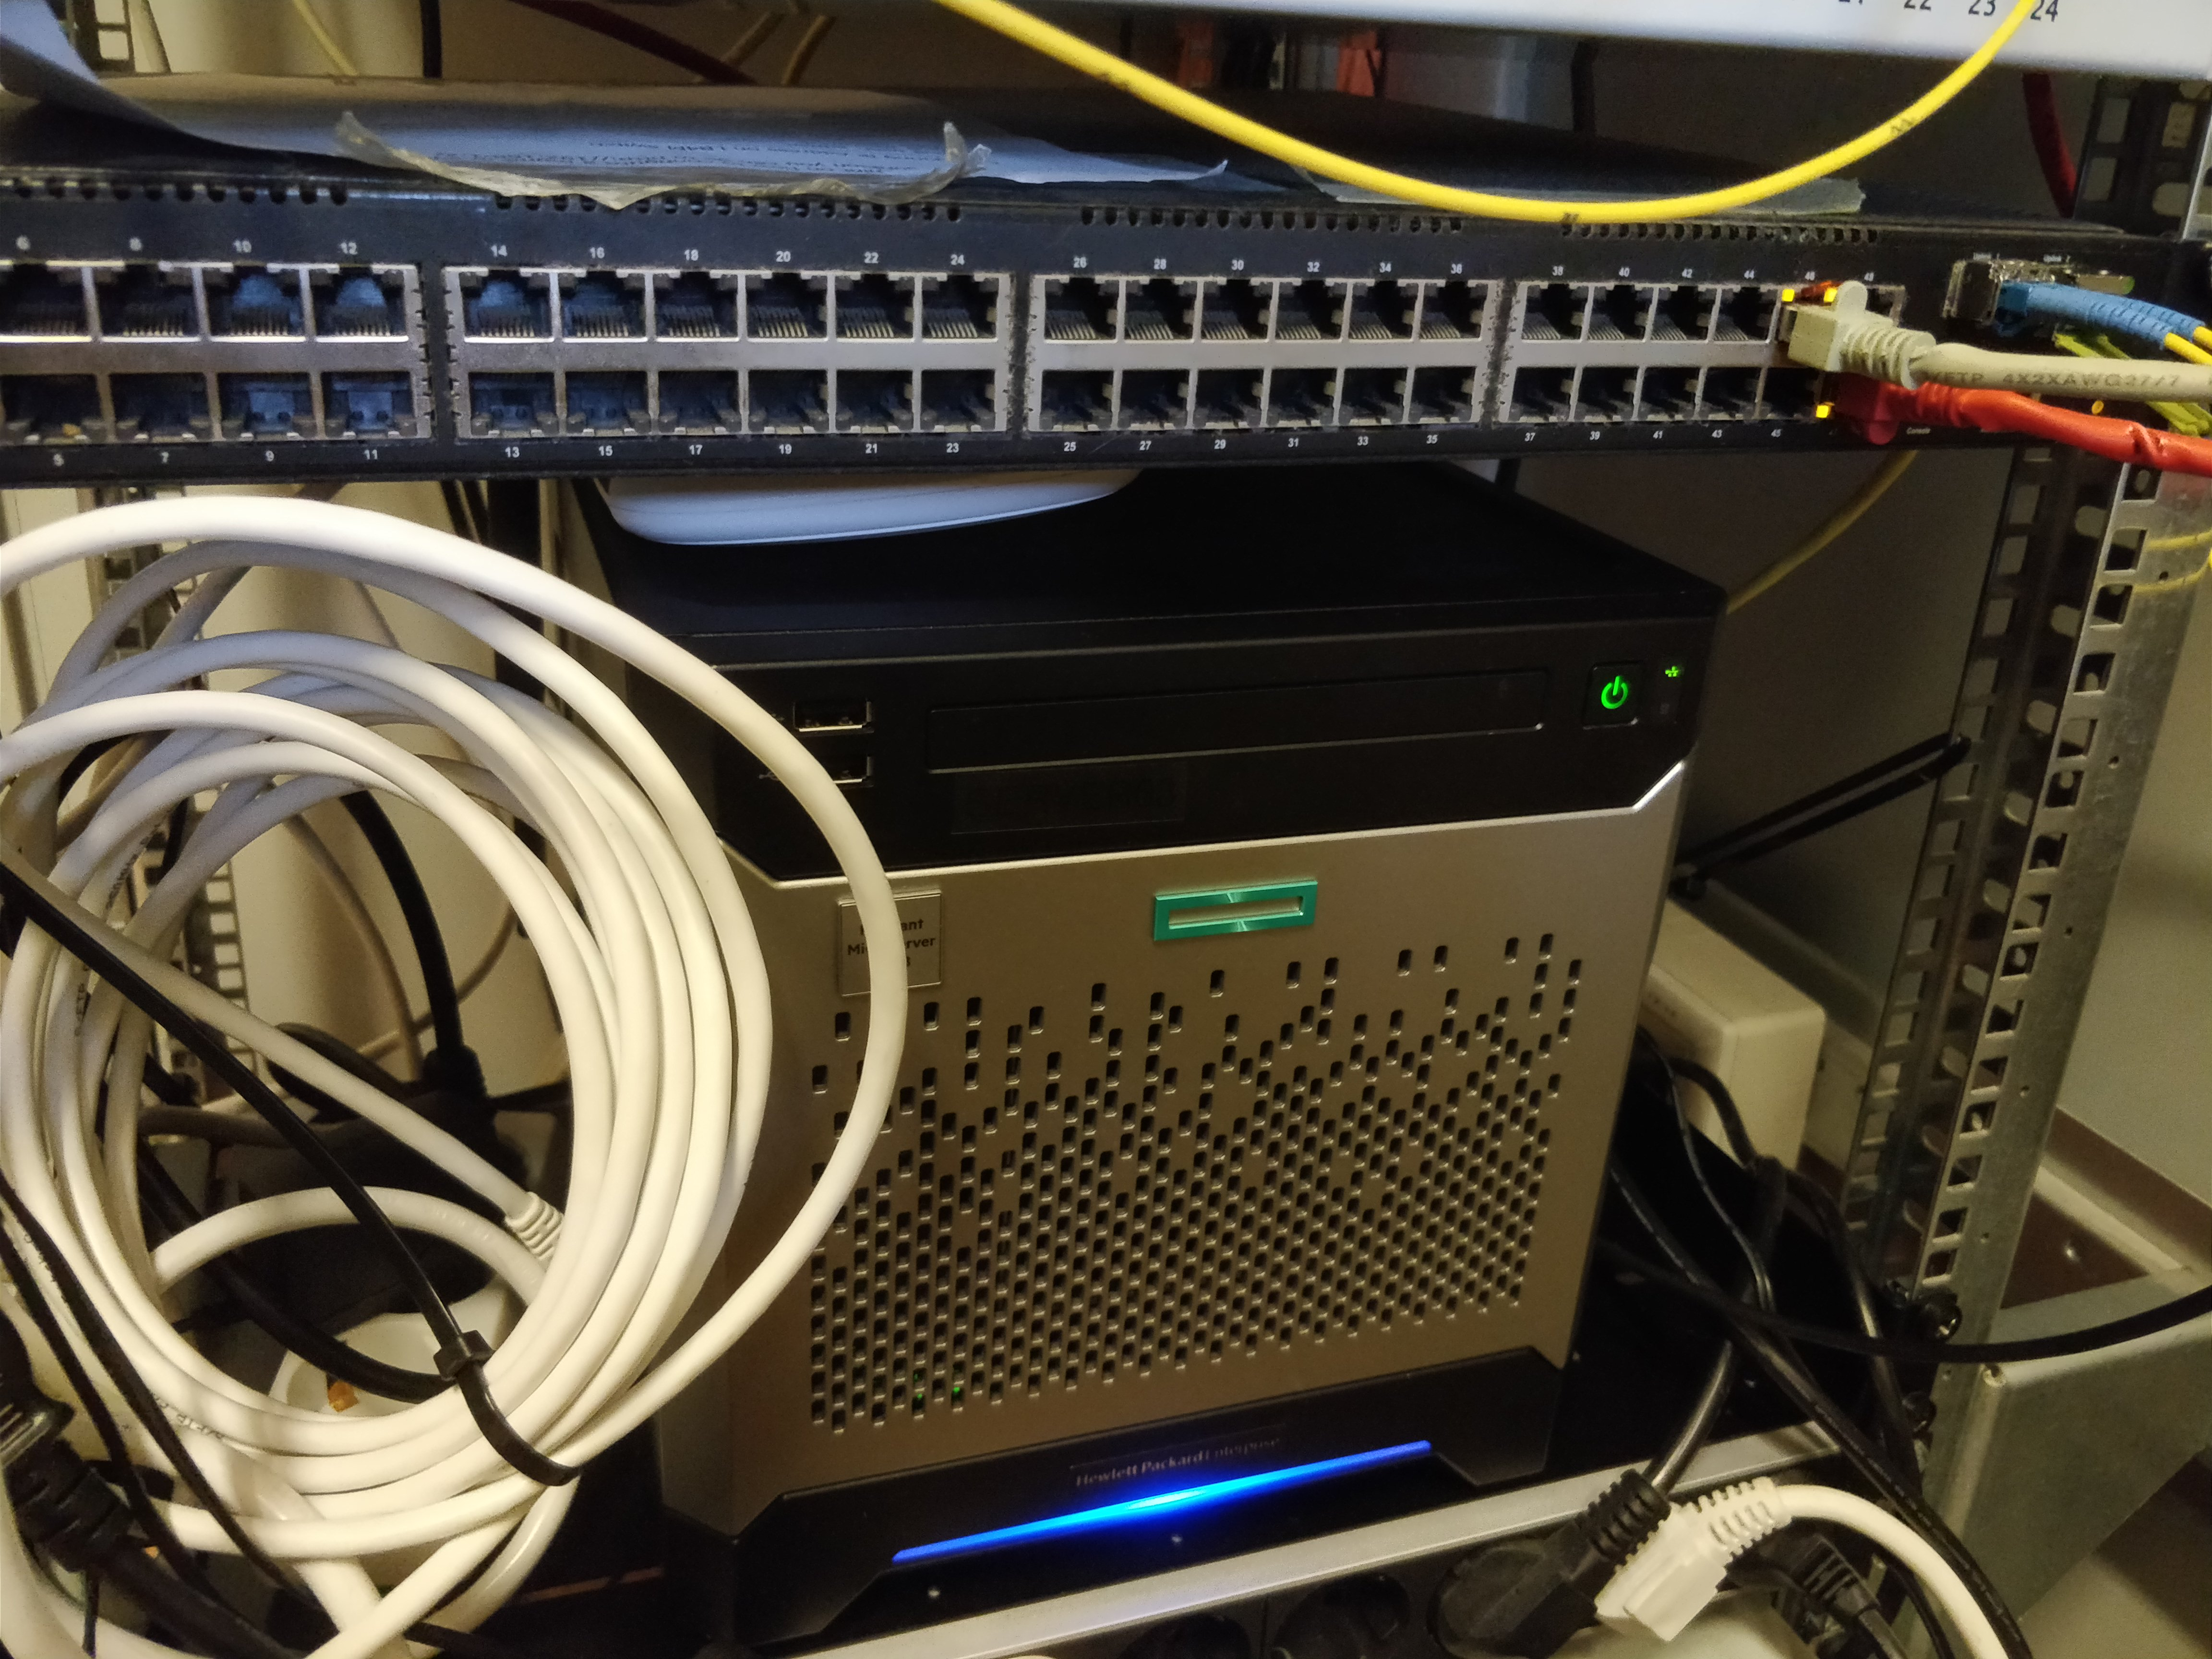
\includegraphics[height=0.86\textheight]{img/zbau-server}
    }
    \only<3>{
        \center
        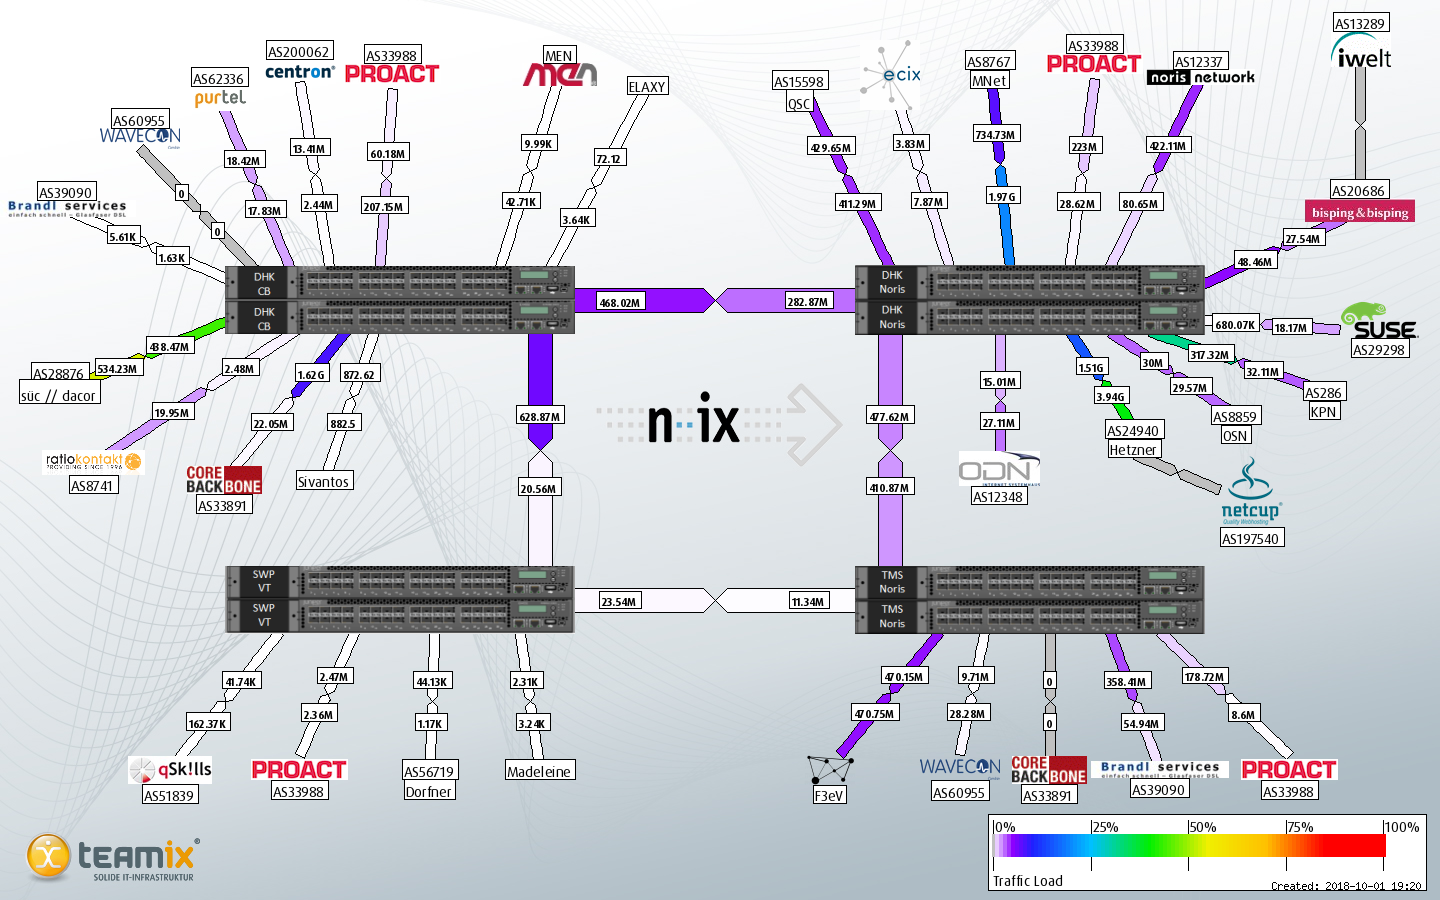
\includegraphics[height=0.86\textheight]{img/NIX}
    }
\end{frame}

\begin{frame}{Gemeinnützigkeit}
    \begin{columns}[T]
        \begin{column}{0.6\textwidth}
            \begin{itemize}
                \item Gemeinnützigkeit noch nicht anerkannt
                \item Verfahren pausiert
                \item Laut AEAO Liste aus §52 Absatz 2 Satz 1
                \item Laut AEAO ''Internetvereine'' per se nicht gemeinnützig
            \end{itemize}
        \end{column}
        \begin{column}{0.35\textwidth}
            
\includegraphics[width=\textwidth]{img/betterplace}
        \end{column}
    \end{columns}

    \vfill

    $\rightarrow$ Help needed\\
    \url{https://www.betterplace.org/de/projects/60168}

    \vfill
\end{frame}



\begin{frame}{Ende}
    \begin{center}
        Vielen Dank für eure Aufmerksamkeit!\\
        \vfill
        Viel Spass auf dem Festival
     \end{center}
\end{frame}\addtocounter{framenumber}{-1}

%%%%%%%%%%%%%%%%%%%%%% /CONTENT %%%%%%%%%%%%%%%%%%%%%%%%%%%%

\end{document}
